\documentclass[tikz,border=1pt]{standalone}
\usepackage{lmodern}\renewcommand{\familydefault}{\sfdefault}\usepackage[T1]{fontenc}
\usetikzlibrary{arrows.meta,positioning,calc}
\definecolor{ink}{HTML}{1A1A1A}\definecolor{gr}{HTML}{8A8A8A}\definecolor{grf}{HTML}{F2F2F2}
\definecolor{or}{HTML}{D55E00}\definecolor{orf}{HTML}{FDEEE6}\definecolor{gn}{HTML}{009E73}\definecolor{gnf}{HTML}{E6F5F0}
\definecolor{panel}{HTML}{FAFAFA}\definecolor{pline}{HTML}{C8C8C8}
\tikzset{
  box/.style={draw=gr,fill=grf,line width=0.6pt,rounded corners=2pt,minimum width=2.95cm,text width=2.8cm,minimum height=1.55cm,align=center,inner sep=2pt,font=\footnotesize,text=ink},
  mukv/.style={box,draw=or,fill=orf,line width=0.8pt},
  wide/.style={box,minimum width=7.6cm,text width=7.4cm,minimum height=1.2cm},
  wmukv/.style={wide,draw=or,fill=orf,line width=0.8pt},
  data/.style={-{Stealth[length=4pt,width=3.5pt]},line width=0.6pt,ink},
  ctrl/.style={-{Stealth[length=4pt,width=3.5pt]},line width=0.6pt,or,dashed},
  ctrlg/.style={-{Stealth[length=4pt,width=3.5pt]},line width=0.6pt,gr,dashed},
  heat/.style={-{Stealth[length=4pt,width=3.5pt]},line width=0.7pt,gr,dotted},
  meas/.style={-{Stealth[length=4pt,width=3.5pt]},line width=0.6pt,gn,dash dot},
  lab/.style={font=\scriptsize,inner sep=1pt,text=ink},
  stepn/.style={circle,fill=or,text=white,font=\bfseries\tiny,inner sep=1pt,minimum size=9pt},
  stepg/.style={stepn,fill=gr},
  stepr/.style={rectangle,rounded corners=3pt,fill=or,text=white,font=\bfseries\tiny,inner sep=1.5pt,minimum height=9pt},
  head/.style={font=\bfseries\scriptsize,inner sep=1pt}
}
\newcommand{\bx}[2]{\textbf{#1}\\[1pt]{\scriptsize #2}}
\begin{document}
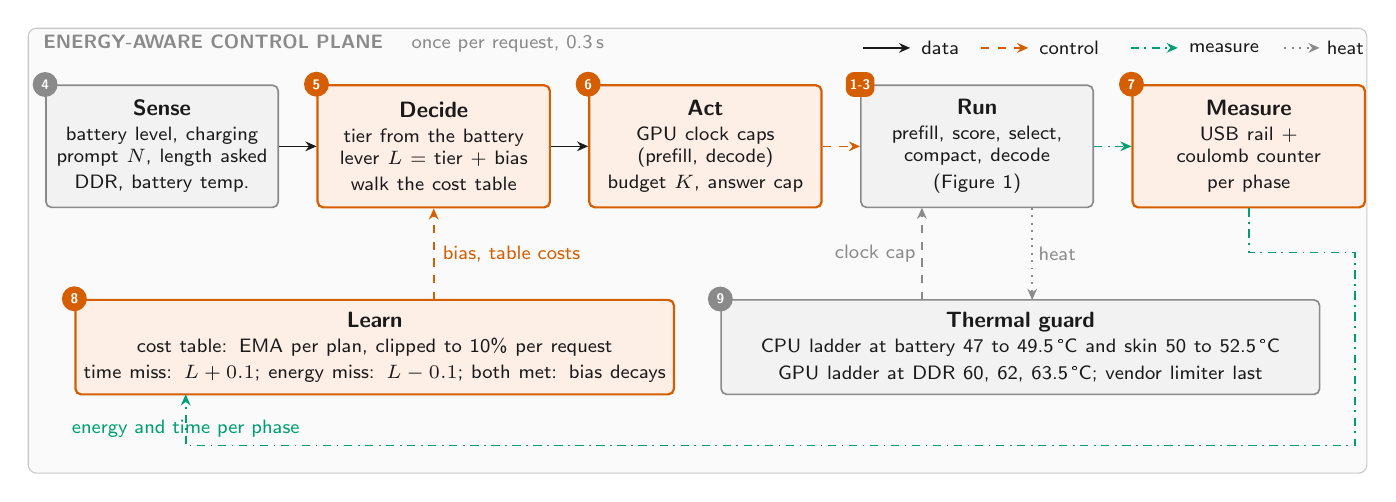
\begin{tikzpicture}[x=1cm,y=1cm]
\fill[panel,draw=pline,rounded corners=3pt] (0,-0.45) rectangle (17,5.2);
\node[head,anchor=north west,text=gr] at (0.15,5.15) {ENERGY-AWARE CONTROL PLANE \quad {\mdseries once per request, 0.3\,s}};
% legend in the title row
\draw[data] (10.6,4.95) -- (11.2,4.95);\node[lab,anchor=west] at (11.3,4.95) {data};
\draw[ctrl] (12.1,4.95) -- (12.7,4.95);\node[lab,anchor=west] at (12.8,4.95) {control};
\draw[meas] (14.0,4.95) -- (14.6,4.95);\node[lab,anchor=west] at (14.7,4.95) {measure};
\draw[heat] (15.95,4.95) -- (16.4,4.95);\node[lab,anchor=west] at (16.45,4.95) {heat};
% ring, five boxes
\node[box]  (sense)   at (1.7,3.7) {\bx{Sense}{battery level, charging\\ prompt $N$, length asked\\ DDR, battery temp.}};
\node[mukv] (decide)  at (5.15,3.7)  {\bx{Decide}{tier from the battery\\ lever $L$ = tier + bias\\ walk the cost table}};
\node[mukv] (act)     at (8.6,3.7) {\bx{Act}{GPU clock caps\\ (prefill, decode)\\ budget $K$, answer cap}};
\node[box]  (run)     at (12.05,3.7) {\bx{Run}{prefill, score, select,\\ compact, decode\\ (Figure~1)}};
\node[mukv] (measure) at (15.5,3.7){\bx{Measure}{USB rail +\\ coulomb counter\\ per phase}};
\node[stepg] at (sense.north west) {4};\node[stepn] at (decide.north west) {5};\node[stepn] at (act.north west) {6};
\node[stepr] at (run.north west) {1-3};\node[stepn] at (measure.north west) {7};
\draw[data] (sense) -- (decide);
\draw[data] (decide) -- (act);
\draw[ctrl] (act) -- (run);
\draw[meas] (run) -- (measure);
% learn and thermal guard
\node[wmukv] (learn) at (4.4,1.15) {\bx{Learn}{cost table: EMA per plan, clipped to 10\% per request\\ time miss: $L+0.1$; energy miss: $L-0.1$; both met: bias decays}};
\node[wide]  (guard) at (12.6,1.15) {\bx{Thermal guard}{CPU ladder at battery 47 to 49.5\,\textdegree C and skin 50 to 52.5\,\textdegree C\\ GPU ladder at DDR 60, 62, 63.5\,\textdegree C; vendor limiter last}};
\node[stepn] at (learn.north west) {8};\node[stepg] at (guard.north west) {9};
\draw[meas] (measure.south) -- (15.5,2.35) -- (16.85,2.35) -- (16.85,-0.1) -- (2.0,-0.1) -- (2.0,0.55) node[lab,text=gn,pos=0.62,below=1pt] {energy and time per phase};
\draw[ctrl] (5.15,1.75) -- (decide.south) node[lab,text=or,pos=0.5,right=2pt] {bias, table costs};
\draw[heat] (12.75,2.92) -- (12.75,1.75) node[lab,text=gr,pos=0.5,right=1pt] {heat};
\draw[ctrlg] (11.35,1.75) -- (11.35,2.92) node[lab,text=gr,pos=0.5,left=1pt] {clock cap};
\end{tikzpicture}
\end{document}
